\chapter{Framework EPUBKit}
\section{Tworzenie frameworku na iOS}

Tworzenie bilioteki którą zamierzamy następnie wykorzystać we własnej aplikacji lub udostępnić publiczne, jest stosunkowo prostym procesem. Wszystko sprowadza się do stworzenia nowego projektu w Xcode a następnie dołączenie go do przestrzeni roboczej (Xcode Workspace) w której znajdzie się projekt aplikacji nad którą pracujemy oraz projekt biblioteki. Aby stworzyć projekt biblopteki należy uruchomić Xcode IDE i na powitalnym ekranie wybrać opcję "Create a new Xcode project" która przeniesie nas do kolejnego ekranu z możliwością wybrania konktetnego szablonu projektu nad jakim chcemy pracować.

\begin{figure}[ht!]
  \centering
  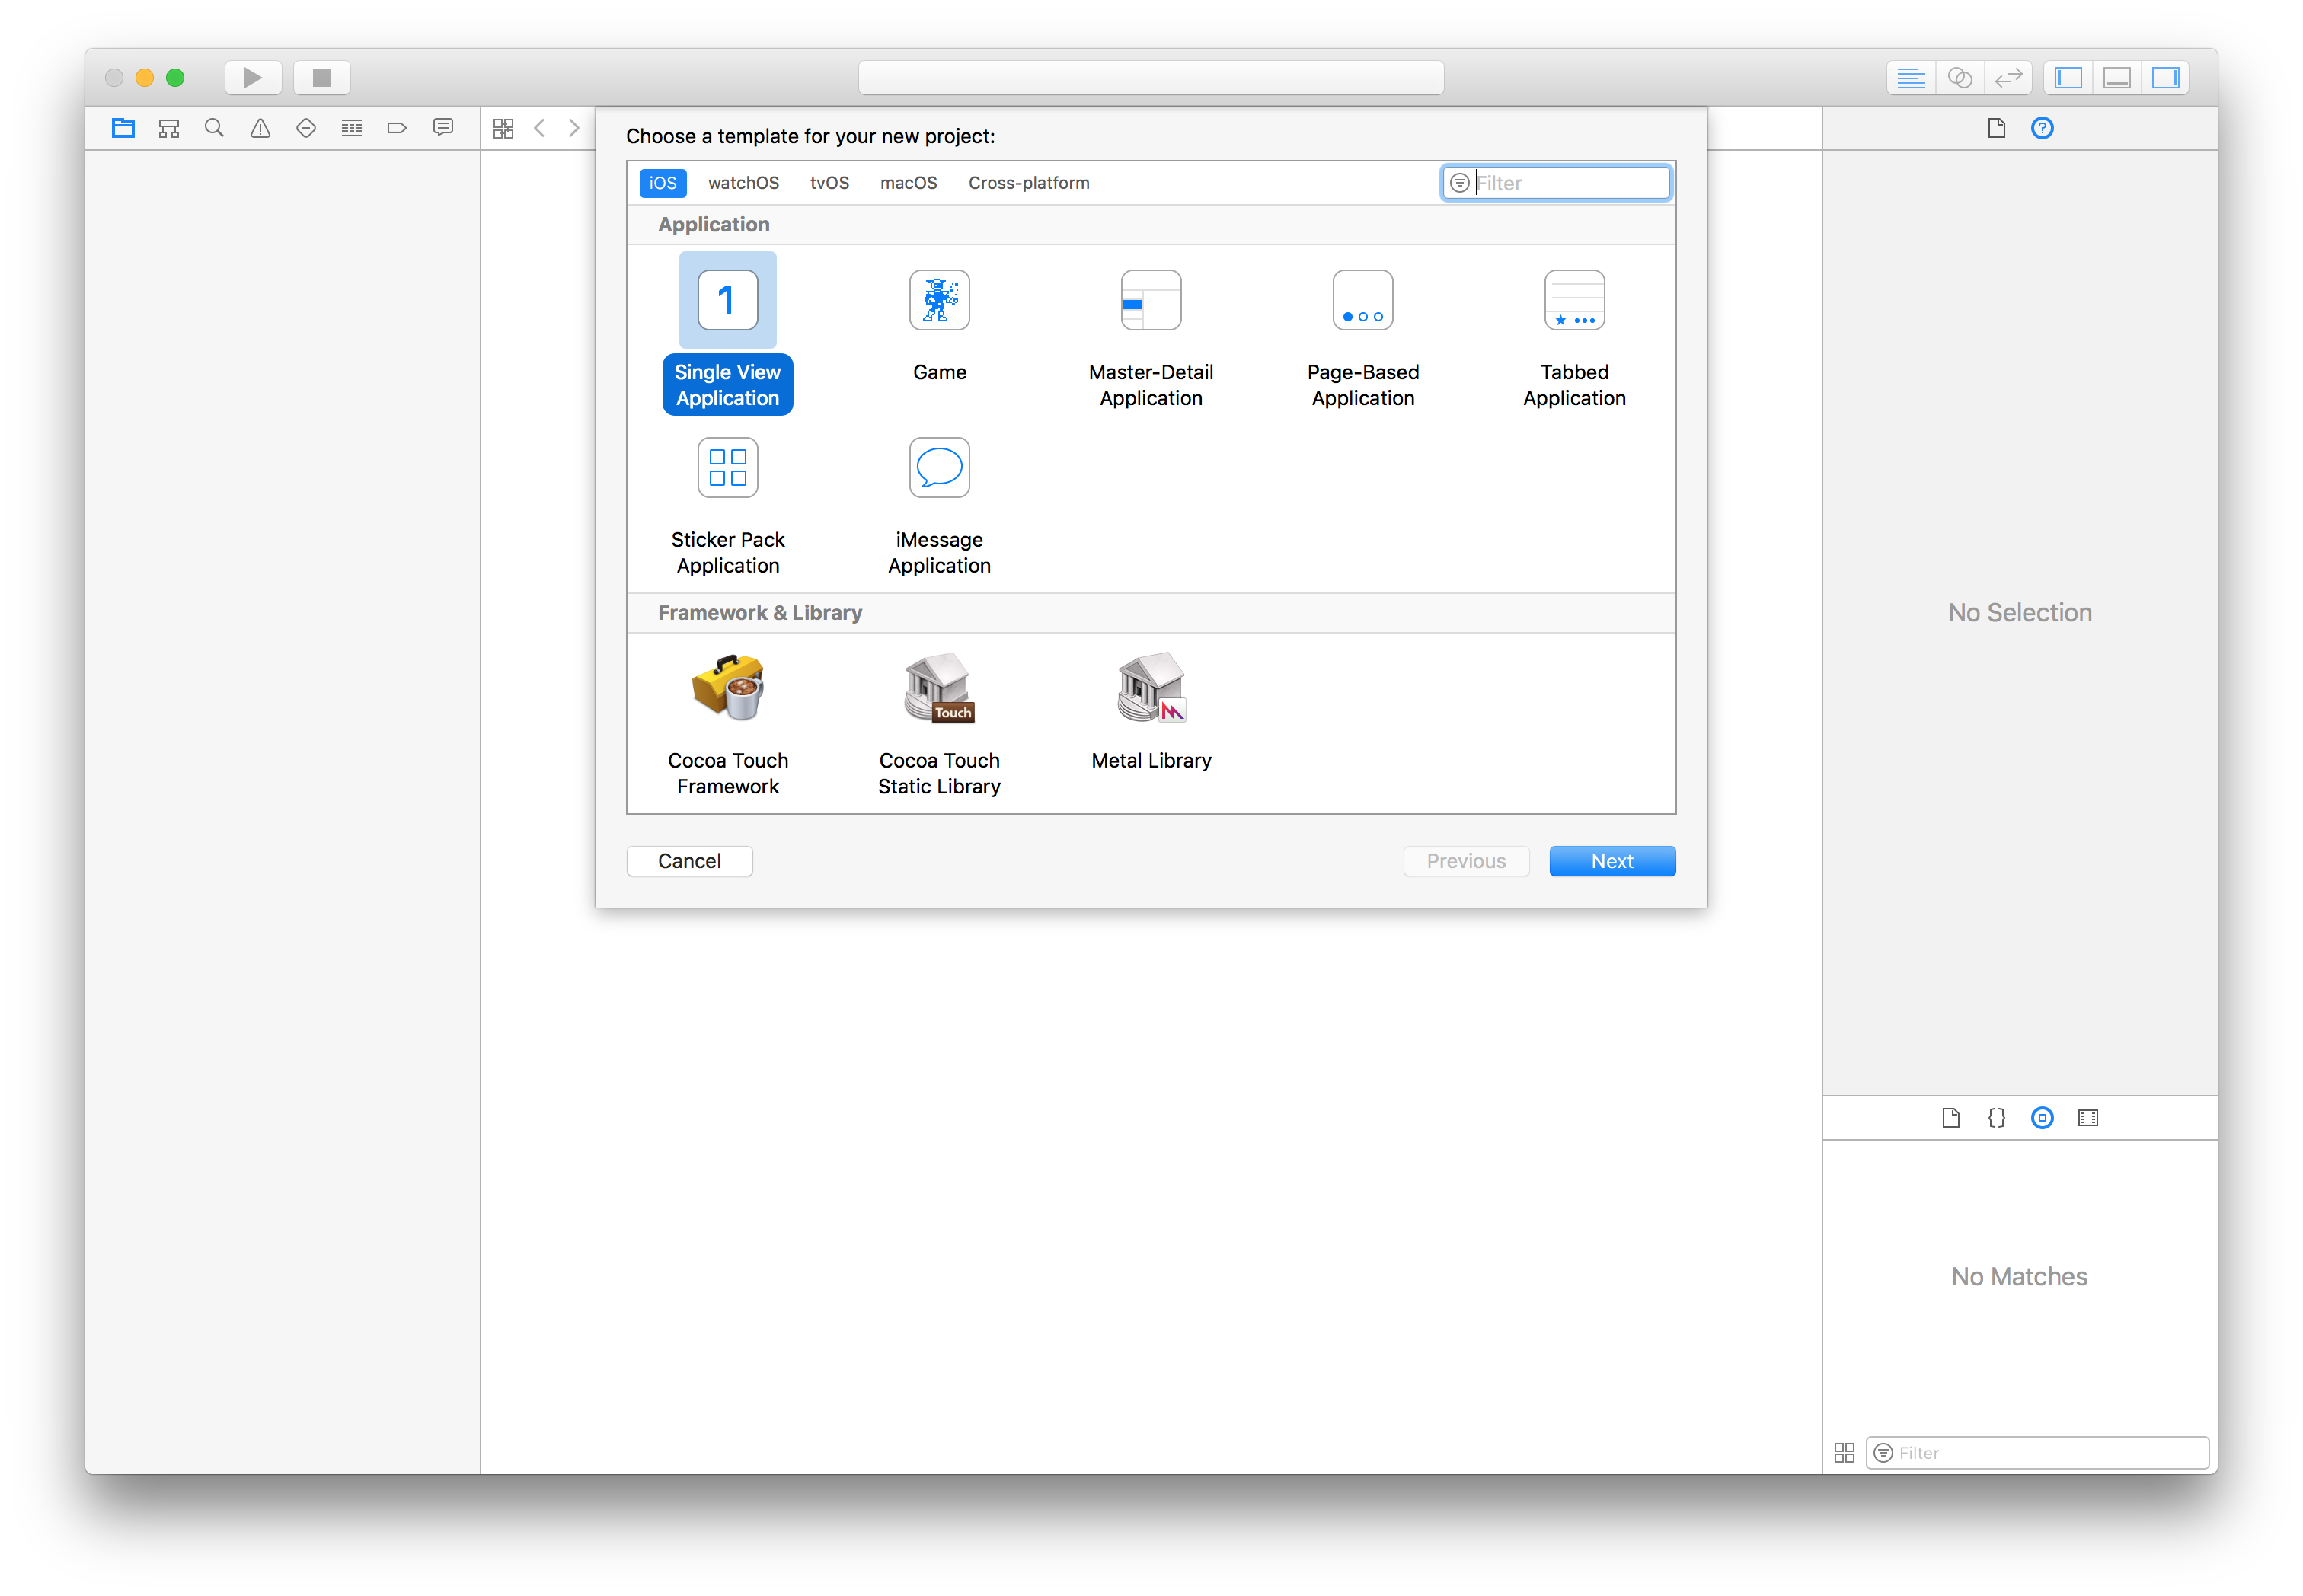
\includegraphics[width=120mm]{images/chapter-4-image-1-new-project.png}
  \caption{Szablny projektów które znajdują się w Xcode}
  \label{chapter-4-image-1-new-project}
\end{figure}

Na naszym przypadku interesuje nas szablon "Cocoa Touch Framework", a po jego wybraniu jesteśmy proszeni o uzupełnienie formularza ze szczegółowymi informacjami na temat projektu który zamierzamy stworzyć, poczynając od nazwy, po język w którym będzie napisany (Swift lub Objective-C). Następnie Xcode poprosi o wskazanie lokalizacji na dysku w której chcemy zapisać projekt oraz zapyta nas czy chcemy stworzy repozytorium systemu kontroli wersji git. W tym momencie mamy projekt który można już w prosty sposób dołączyć do aplikacji (Co zostanie opisane w kolejnym rozdziale przy okazji omawianie wykorzystania biblioteki EPUBKit w demonstracyjnej aplikacji). Teraz już możemy tworzyć klasy które mają składać sie na funkcjonalność biblioteki.

\begin{figure}[ht!]
  \centering
  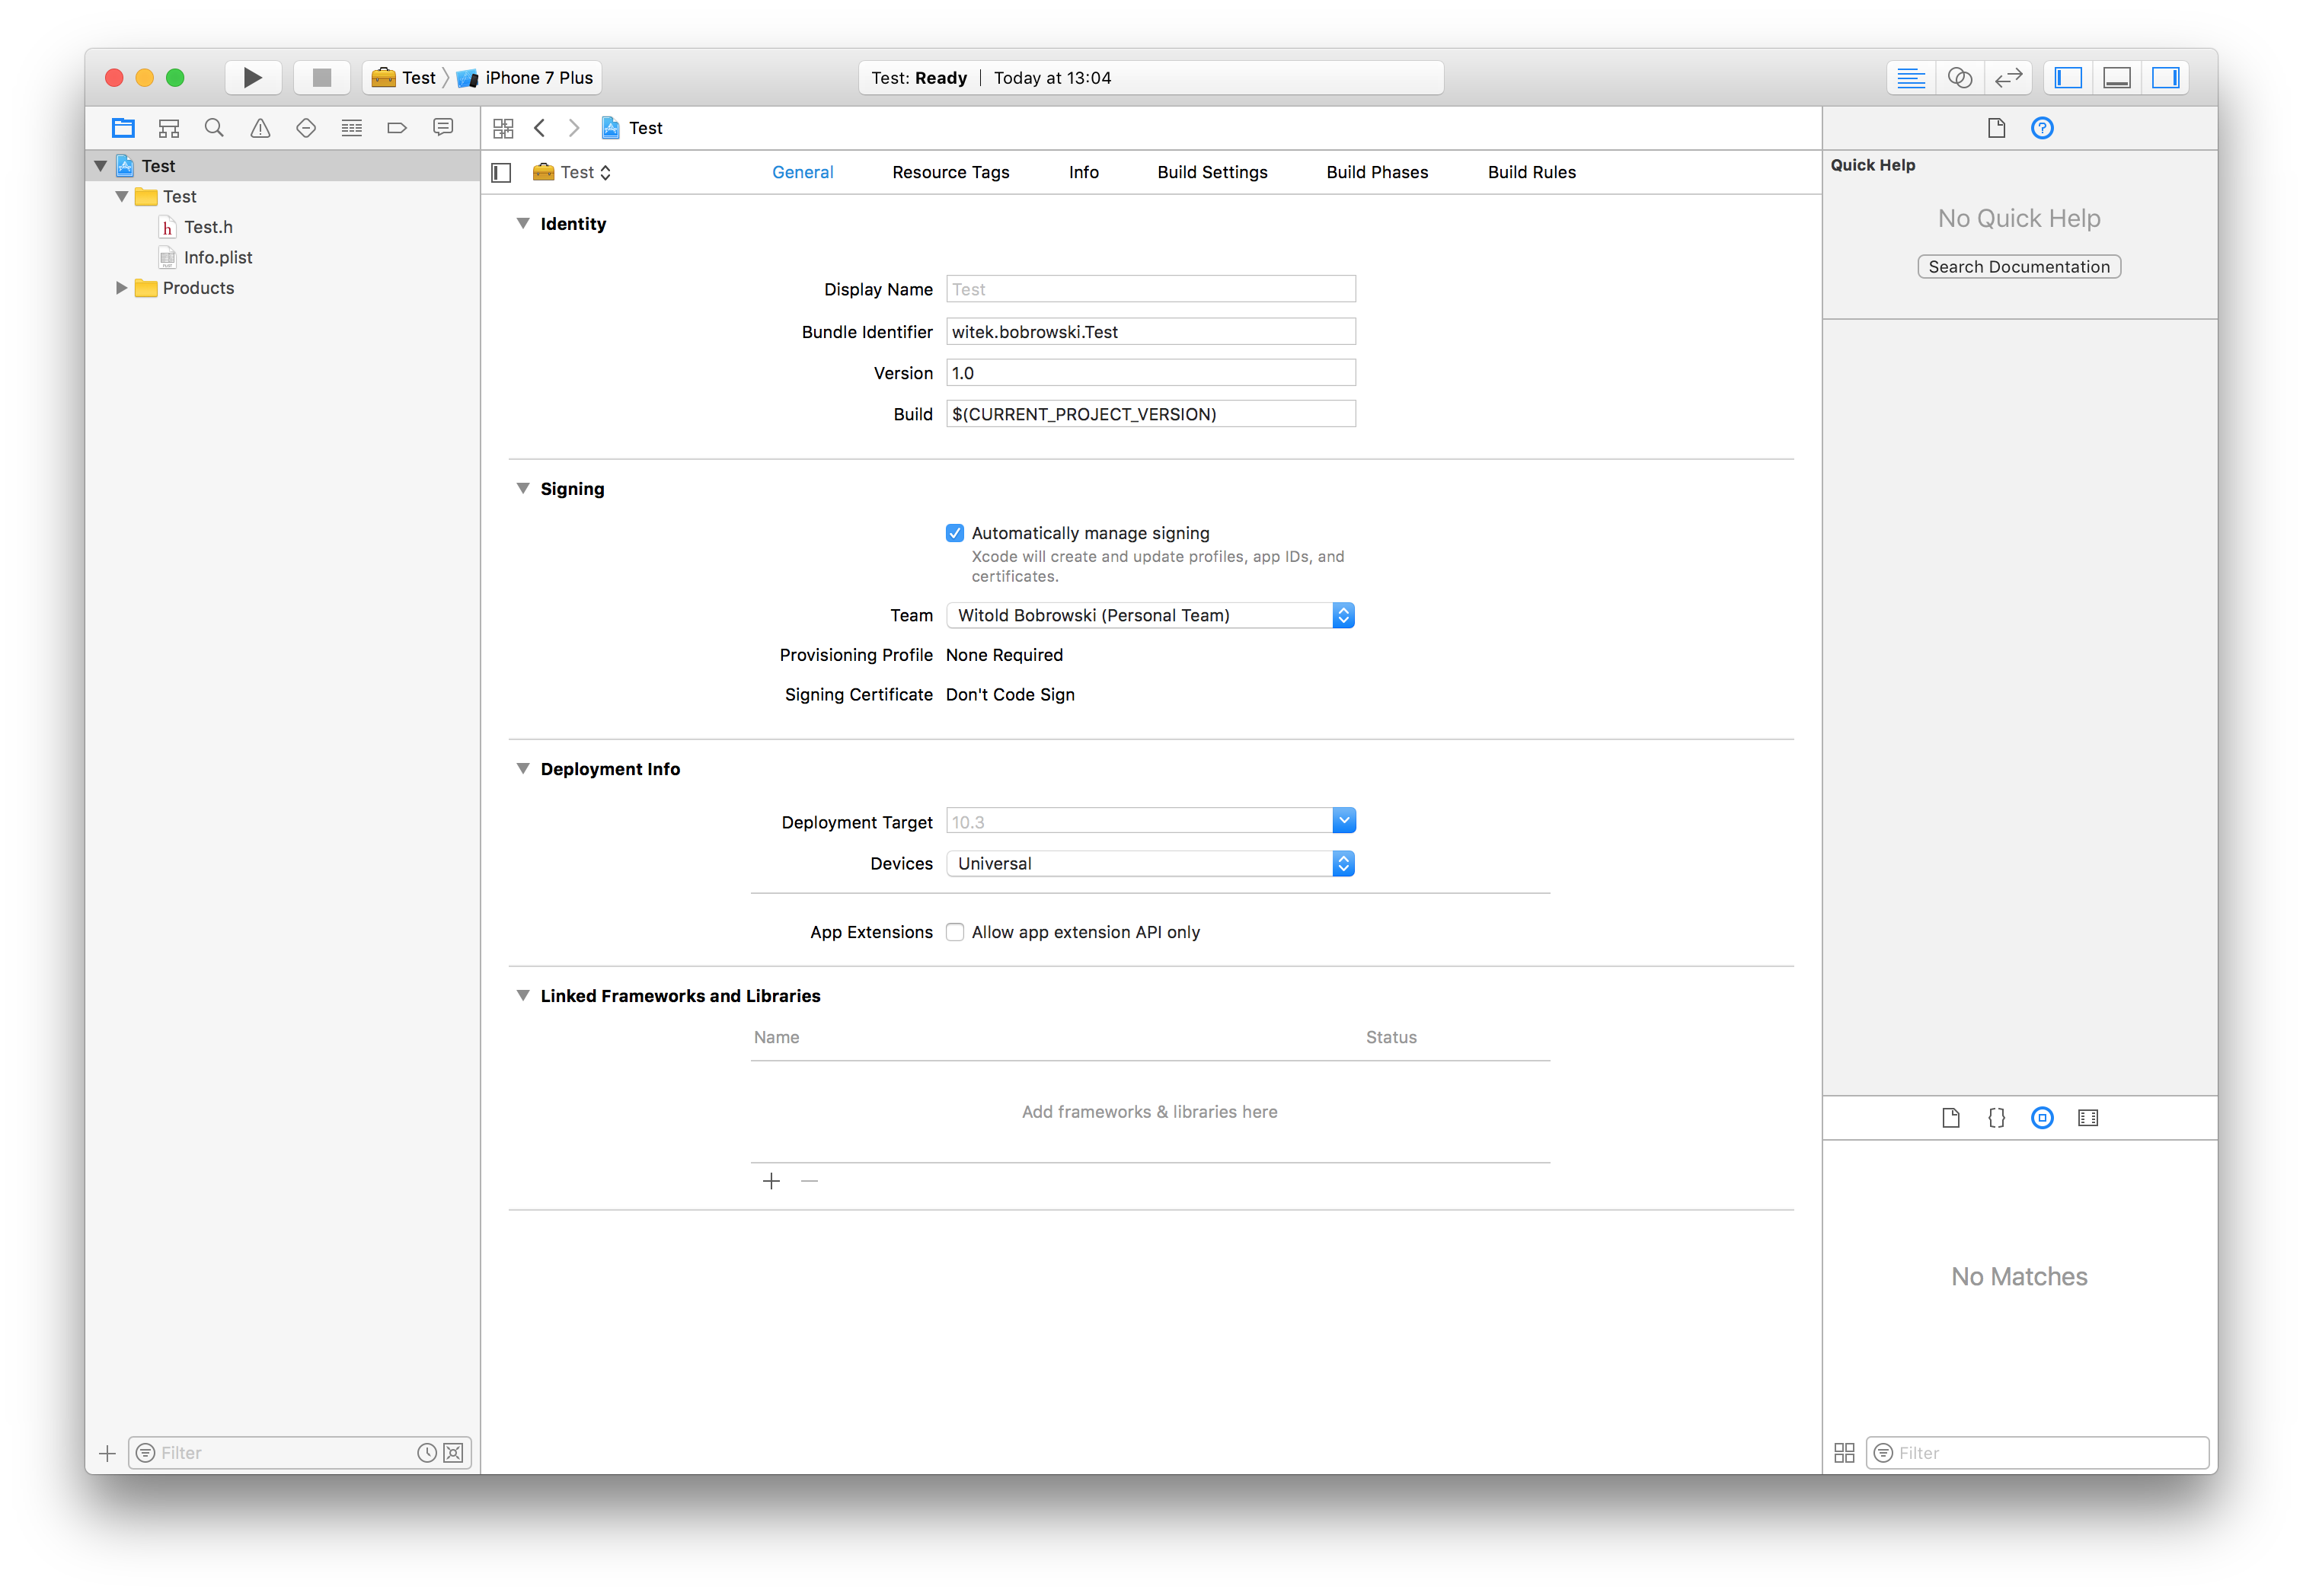
\includegraphics[width=120mm]{images/chapter-4-image-2-empty-project.png}
  \caption{Szablny projektów które znajdują się w Xcode}
  \label{chapter-4-image-2-empty-project}
\end{figure}

Plik projektu pozwala nam za szczegółowy wgląd w preferencje oraz infromacje jego dotyczące, które można zmieniac w dowolnej chwili. Jest możliwość zmiany wersji bibioteki, docelowego urządzenia (iPhone lub iPad), preferowanej wersji systemu który ma wspierać bibltioteka, oraz co bardzo istotne, mamy możliwość użycia innych niezależnych bibliotek w naszym projekcie. Wystarczy wyeksportować plik projektu jako plik przestrzebi roboczej do której można dodać inne projekty a następnie połączyć je z naszym w menu "General" w polu "Linked Frameworks and Libraries" w pliku projektu. Dzięki tak funkcjonalnym i prostym w obsłudze narzędziom jak Xcode, po szybkiej konfiguracji swoją uwagę można skupić na samej logice którą chcemy zaimplementować.

W tym rozdziale zostanie opisana stworzna przez mnie biblioteka EPUBKit. Biblioteka ta jest oparta na architekturze MVC (Model View Controller) dlatego omówienie jest rozpocznę od opisania jej modelu oraz parsera, a następnie przejdę do zawartych w niej widokach które pozwalają na wyświetlenie danych zawartych w modelu. Zakończę rozdział przedstawiając możliwości dystrybuowania takiej biblioteki, przy pomocy szeroko stosowanych i popularnych narzędzi, które są podstawą iOS developmentu.

\section{Model}

Struktura klas modelu została zaprojektowana w ten sposób aby z jednej strony odzwierciedlała struktrę dokumnetu EPUB oraz format OPF który EPUB wykorzystuje, a z drugiej by trzymała się konwencji swiftowych i intuicyjnie reprezontowała obiekt który następnie będzie wykorzystywany w kolejnych klasach biblioteki.

\begin{lstlisting}[caption={Struktura modelu EPUBKit.}, language=bash]
    Model
    |-- EPUBDocument.swift
    |-- EPUBManifest.swift
    |-- EPUBMetadata.swift
    |-- EPUBSpine.swift
    `-- EPUBTableOfContents.swift
\end{lstlisting}

\subsection{EPUBDocument}

EPUBDocumnet jest klasą publiczną reprezentującą całą poblikację EPUB i agregującą pozostałe struktury modelu biblioteki jako jej stałe własności (ze względu na nomenklaturę stosowaną w języku Swift, 'properties' będą nazywane własnościami). W języku Swift odróżniamy dwa rodzaje własności, są to stałe (słowo kluczowe let) do których wartość może zostać przypisana wyłącznie jednokrotnie oraz zmienne (słowo kluczowe var) których wartość może być modyfikowana w dowolnym momencie.

\begin{lstlisting}[caption={Deklaracje własności w Swifcie.\cite{theSwiftProgrammingLanguagePropertyDefinition}}, language=swift-reference]
  let (constant name): (type) = (expression)
  var (variable name): (type) = (expression)
\end{lstlisting}

Własności zostały oznaczone jako stałe ze względu na statyczną naturę struktury publikacji EPUB. Ciężko sobie wyobracić powód dla którego któreś z metadanych publikacji miały by zostać zmienione albo któreś z dokumentów XML usunięte z manifestu publikacji. Dlatego biorąc pod uwagę kontekst, w którym klasa się znajduje, zdecydowałem się oznaczenie jej własności jako stałe aby zapewnić klasie niemodalność oraz zgodność z wytycznymi odnośnie projektowania klas i struktór w języku Swift według których powinno oznaczać się własności jako stałe w każdej sytuacji która nie wymaga od nas ich mutowania, a słowa "mutowania" użyłem tutaj nie bez powodu, co stanie się jasne w kolejnym akapicie.

\begin{lstlisting}[caption={Klasa EPUBDocument i jej stałe publiczne.}, language=swift]
public class EPUBDocument {
    public let directory: URL
    public let contentDirectory: URL
    public let metadata: EPUBMetadata
    public let manifest: EPUBManifest
    public let spine: EPUBSpine
    public let tableOfContents: EPUBTableOfContents
}
\end{lstlisting}

W przeciwieństwie do C, struktury w Swiftcie mogą posiadać metody. W przypadku gdy metoda w jakiś sposób zmiania własności musi ona zostać oznaczona słowem kluczowym 'mutating' co tyczy się również metod enumeracji. Wspominam o tym, ponieważ chciałbym wytłumaczyc dlaczego typy własności klasy EPUBDocument są strukturami a nie klasami. Ze względu na to, że instancje klasy są przekazywane przez referencję, a instancje struktur są przekazywane przez kopiowanie wartości, oznacz to że są one przeznaczone do innych zadań. Zgodnie z wytycznymi Apple, strukturami powinno oznaczać się typy, których zadaniem jest enkapsulacja relatywnie prostych wartości\cite{theSwiftProgrammingLanguageStructsPurpose}, co jest prawdą w przypadku wcześniej wspomnianych typów (zostaną one opisane w kolejnych paragrafach).

Klasa EPUBDocument posiada dwa inicjalizatory które pozwalają tworzyć instancje tej klasy. Pierwszym z nich jest inicjalizator prywatny w nomenklaturze swiftowej "memberwise initialiser" ze względu na kolejność argumentów które przyjmuje, która zgodna jest z kolejnością deklajacji własności. Inicjalizator ten został oznaczony jako prywatny ponieważ jego przeznaczeniem jest inicjalizować instancję jedynie przy pomocy drugiego inicjalizatora. Drugi z inicjalizatorów jest dostępny publicznie, i jest jedynym publicznym inicjalizatorem dla tej klasy.

\begin{lstlisting}[caption={Inicjalizatory klasy EPUBDocument.}, language=swift]
private init (directory: URL, contentDirectory: URL, metadata: EPUBMetadata, manifest: EPUBManifest, spine: EPUBSpine, toc: EPUBTableOfContents) {
    self.directory = directory
    self.contentDirectory = contentDirectory
    self.metadata = metadata
    self.manifest = manifest
    self.spine = spine
    self.tableOfContents = toc
}

public convenience init?(named: String) {
    let parser = try? EPUBParser(named: named)
    guard let directory = parser?.directory,
        let contentDirectory = parser?.contentDirectory,
        let metadata = parser?.metadata,
        let manifest = parser?.manifest,
        let spine = parser?.spine,
        let tableOfContents = parser?.tableOfContents else { return nil }
    self.init(directory: directory, contentDirectory: contentDirectory, metadata: metadata, manifest: manifest, spine: spine, toc: tableOfContents)
}
\end{lstlisting}

Zważając na naturę publikacji EPUB jako spójnej całości, zdecydowałem ograniczyć się inicjalizowanie klasy EPUBDocument do inicjalizatora pomocniczego, który wykorzystuje do tego parser. Ten inicjalizator wykorzystuje w pełni możliwości Swifta. Oznaczając go słowem kluczowym "convenience", zmuszam go do wykorzystania wyznaczonego (z ang. designated) inicjalizatora ponieważ pomocniczy inicjalizator nie może samemu tworzyć instancji, musi do tego wykorzystać wyznaczony inicjalizator (w tym przypadku jest to pierwszy inicjalizator, który jest prywatny). Dodatkowo pomocniczy inicjalizator, jest oznaczony znakiem zapytania "init?" co oznacza, że inicjalizacje może się niepowieść, a w takiej sytuacji inicjalizator zwróci... nic, czyli "nil" w Swifcie. Konsekwencją tego jest to, że typ która zwraca ten inicjalizator to "EPUBDocument?" a nie "EPUBDocument", co oznacza że może on nie mieć żadnej wartości co trzeba w odpowiedni sposób obsłużyć. Przeanalizujmy więc krok po kroku operacje, które wykonuje inicjalizator pomocniczy.

\begin{lstlisting}[language=swift-reference]
    let parser = try? EPUBParser(named: named)
\end{lstlisting}

Na wstępie tworzy instancję parsera, i jako argument inicjalizatora podaje własny parametr który wskazuje na nazwę publikacji EPUB. Słowo kluczowe "try" onacza, że inicjalizator może zwrócić błąd, a dzięki znakowi zapytania błąd ten gdy zostanie rzucony, będzie interpretowany jako zwrócenie nila przez inicjalizator. W ten sposób unikamy umieszczenia bloku "do-catch" co znacznie upraszcza kod. Końcowo znajdujemy się w posiadaniu stałej "parser", która jest typu "EPUBParser?" czyli opcjonalny EPUBParser.

\begin{lstlisting}[language=swift-reference]
  guard let directory = ... else { return nil }
\end{lstlisting}

Wyrażenie "guard let" jest jednym ze sposobów obsłużenia typu opcjonalnego. Jest to odmiana wyrażenia "if let" które pozwala nam na przypisanie wartości zmiennej a, do nowej stałej b, jeżeli zmienna a takową posiada. Wadą takiego rozwiązania jest to, że nowo powstała zmienna b, znajduje się jedynie w zasięgu bloku "if", co w pewien sposób ogranicza dostęp do niej. Z pomocą przychodzą wyrażenia "guard", dzięki który zadeklarujemy nową stałą, która będzie przyjmowała wartość zmiennej, którą chcemy "rozpakować" (z ang. unwrap, co odnosi się do czynności wywłaszczania wartości z typu opcjonalnego) i będzie ona dostępna w obrębie tego samego bloku co wyrażenie guard. Dodatkowo mamy możliwość wykonania jakiejść czynności w sytuacji gdy zmienna którą rozpakowywujemy nie ma wartości, co w tym konkretnym przypadku będzie oznaczało niepowodzenie wywłaszczenia którejś z wartości parsera a więc inicjalizator EPUBDocument zwróci nil. Ponieważ wyrażenie "guard" działa w podobny sposób co "if", otrzymuje on również te same funkcjonalności co "if" w Swifcie, czyli możliwość kolejkowania wyrażeń zwracających wartość boolowską (wypisujemy je kolejno po przecinku), i w przypadku zwrócenia fałszu przez jedno z nich, instrukcja natychmiast zostaje przerwana a pozostałe wyrażenia nie zostają ewaluowane, a w tym przypadku program przechodzi do bloku "else".

\begin{lstlisting}[language=swift-reference]
    self.init(...)
\end{lstlisting}

Jeżeli udało się wywłaszczyć wszystkie potrzebne wartości z parsera, to można przejść do tworzenia instancji EPUBDocument. Inicjalizator pomocniczy wywołuje inicjalizator wyznaczony, i dokument zostaje pomyślnie stworzony a wszystkie informacie otrzymane dzięki parserowi zostają przypisane na stałe do jednej instancji EPUBDocument. W ten sposób zostaje zachowana niemutowalność instancji, oraz gwarancja, że wszystkie wartości w których posiadaniu znajduje się instancja, pochodzą z jednego źródła, z którego czerpie parser. Działanie samego parsera zostawiam na kolejny podrozdział.

\subsection{EPUBManifest}
\subsection{EPUBMetadata}
\subsection{EPUBSpine}
\subsection{EPUBTableOfContents}


\section{Parser}

\section{Widok}

\section{Dystrybucja}
